\section{Integer linear programming}

An integer linear programming problem is an optimization problem where each variable $x_i$ is an integer: $\ul{x} \in \mathbb{Z}^n$.

\begin{figure}[H]
    \centering
    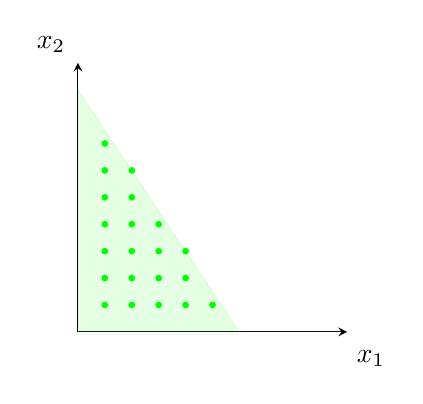
\begin{tikzpicture}
        \begin{axis}[
            axis lines=middle,
            xlabel={$x_1$},
            ylabel={$x_2$},
            xlabel style={at={(axis description cs:1,-0.1)}, anchor=west},
            ylabel style={at={(axis description cs:-0.1,1)}, anchor=south},
            xmin=0, xmax=10,
            ymin=0, ymax=10,
            xtick={0},
            ytick={0},
            domain=0:10,
            samples=10,
            width=5cm, height=5cm
        ]
        \addplot[domain=0:10, color=green, opacity=0.1, fill=green] {-1.5*x + 9} \closedcycle;
        \addplot[only marks, mark=*, green, mark size=1pt] coordinates {(1,1)};
        \addplot[only marks, mark=*, green, mark size=1pt] coordinates {(1,2)};
        \addplot[only marks, mark=*, green, mark size=1pt] coordinates {(1,3)};
        \addplot[only marks, mark=*, green, mark size=1pt] coordinates {(1,4)};
        \addplot[only marks, mark=*, green, mark size=1pt] coordinates {(1,5)};
        \addplot[only marks, mark=*, green, mark size=1pt] coordinates {(1,6)};
        \addplot[only marks, mark=*, green, mark size=1pt] coordinates {(1,7)};
        \addplot[only marks, mark=*, green, mark size=1pt] coordinates {(2,1)};
        \addplot[only marks, mark=*, green, mark size=1pt] coordinates {(2,2)};
        \addplot[only marks, mark=*, green, mark size=1pt] coordinates {(2,3)};
        \addplot[only marks, mark=*, green, mark size=1pt] coordinates {(2,4)};
        \addplot[only marks, mark=*, green, mark size=1pt] coordinates {(2,5)};
        \addplot[only marks, mark=*, green, mark size=1pt] coordinates {(2,6)};
        \addplot[only marks, mark=*, green, mark size=1pt] coordinates {(3,1)};
        \addplot[only marks, mark=*, green, mark size=1pt] coordinates {(3,2)};
        \addplot[only marks, mark=*, green, mark size=1pt] coordinates {(3,3)};
        \addplot[only marks, mark=*, green, mark size=1pt] coordinates {(3,4)};
        \addplot[only marks, mark=*, green, mark size=1pt] coordinates {(4,1)};
        \addplot[only marks, mark=*, green, mark size=1pt] coordinates {(4,2)};
        \addplot[only marks, mark=*, green, mark size=1pt] coordinates {(4,3)};
        \addplot[only marks, mark=*, green, mark size=1pt] coordinates {(5,1)};
        \end{axis}
    \end{tikzpicture}
\end{figure}

The most used methods for solving integer linear programming problems are:

\begin{itemize}
    \item implicit enumeration (branch and bound, dynamic programming), which finds global optima;
    \item cutting planes, which finds global optima;
    \item heuristic algorithms, which finds local optima.
\end{itemize}

\subsection{Branch and bound}

The idea of the branch and bound method is to reduce the problem to a sequence of smaller subproblems, by recursively partitioning the feasible area.

The feasible area $X$ is partitioned in $k$ subsets (branching): $X = X_1 \cup \dots \cup X_k$.
Then, on each partition $X_i$, the subproblem $z_i = \min \{ c(\ul{x}) : \ul{x} \in X_i \}$ is solved (bounding), or it is furthermore partitioned.

\begin{figure}[H]
    \centering
    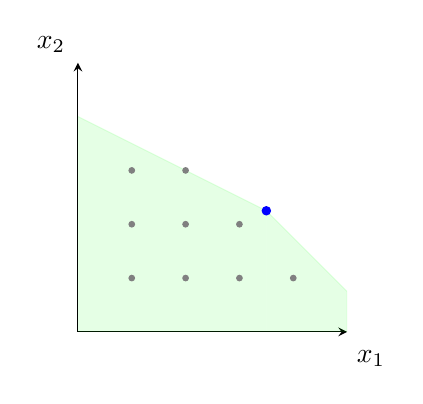
\begin{tikzpicture}
        \begin{axis}[
            axis lines=middle,
            xlabel={$x_1$},
            ylabel={$x_2$},
            xlabel style={at={(axis description cs:1,-0.1)}, anchor=west},
            ylabel style={at={(axis description cs:-0.1,1)}, anchor=south},
            xmin=0, xmax=10,
            ymin=0, ymax=10,
            xtick={0},
            ytick={0},
            domain=0:10,
            samples=10,
            width=5cm, height=5cm
        ]
        \draw[green, opacity=0.1] (axis cs:0,8) -- (axis cs:7,4.5) -- (axis cs:10,1.5) -- (axis cs:10,0);
        \addplot[domain=0:7, color=green, opacity=0.1, fill=green, draw=none] {-0.5*x + 8} \closedcycle;
        \addplot[domain=7:10, color=green, opacity=0.1, fill=green, draw=none] {-x + 11.5} \closedcycle;
        \addplot[only marks, mark=*, gray, mark size=1pt] coordinates {(2,2)};
        \addplot[only marks, mark=*, gray, mark size=1pt] coordinates {(2,4)};
        \addplot[only marks, mark=*, gray, mark size=1pt] coordinates {(2,6)};
        \addplot[only marks, mark=*, gray, mark size=1pt] coordinates {(4,2)};
        \addplot[only marks, mark=*, gray, mark size=1pt] coordinates {(4,4)};
        \addplot[only marks, mark=*, gray, mark size=1pt] coordinates {(4,6)};
        \addplot[only marks, mark=*, gray, mark size=1pt] coordinates {(6,2)};
        \addplot[only marks, mark=*, gray, mark size=1pt] coordinates {(6,4)};
        \addplot[only marks, mark=*, gray, mark size=1pt] coordinates {(8,2)};
        \addplot[only marks, mark=*, blue, mark size=1.5pt] coordinates {(7,4.5)};
        \end{axis}
    \end{tikzpicture}
    \hspace{1in}
    \centering
    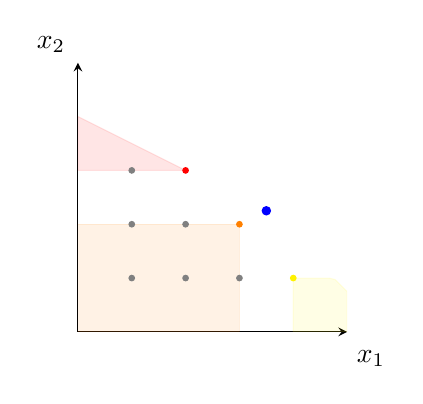
\begin{tikzpicture}
        \begin{axis}[
            axis lines=middle,
            xlabel={$x_1$},
            ylabel={$x_2$},
            xlabel style={at={(axis description cs:1,-0.1)}, anchor=west},
            ylabel style={at={(axis description cs:-0.1,1)}, anchor=south},
            xmin=0, xmax=10,
            ymin=0, ymax=10,
            xtick={0},
            ytick={0},
            domain=0:10,
            samples=10,
            width=5cm, height=5cm
        ]
        \fill[red, opacity=0.1] (axis cs:0,6) -- (axis cs:0,8) -- (axis cs:4,6) -- cycle;
        \draw[red, opacity=0.1] (axis cs:0,6) -- (axis cs:0,8) -- (axis cs:4,6) -- cycle;
        \addplot[domain=0:6, color=orange, opacity=0.1, fill=orange] {min(-0.5*x + 8, 4)} \closedcycle;
        \addplot[domain=8:10, color=yellow, opacity=0.1, fill=yellow] {min(-x + 11.5, 2)} \closedcycle;
        \addplot[only marks, mark=*, gray, mark size=1pt] coordinates {(2,2)};
        \addplot[only marks, mark=*, gray, mark size=1pt] coordinates {(2,4)};
        \addplot[only marks, mark=*, gray, mark size=1pt] coordinates {(2,6)};
        \addplot[only marks, mark=*, gray, mark size=1pt] coordinates {(4,2)};
        \addplot[only marks, mark=*, gray, mark size=1pt] coordinates {(4,4)};
        \addplot[only marks, mark=*, red, mark size=1pt] coordinates {(4,6)};
        \addplot[only marks, mark=*, gray, mark size=1pt] coordinates {(6,2)};
        \addplot[only marks, mark=*, orange, mark size=1pt] coordinates {(6,4)};
        \addplot[only marks, mark=*, yellow, mark size=1pt] coordinates {(8,2)};
        \addplot[only marks, mark=*, blue, mark size=1.5pt] coordinates {(7,4.5)};
        \end{axis}
    \end{tikzpicture}
\end{figure}

\subsection{Cutting planes}

The ideal formulation for an ILP is one where the feasible area has vertices with integer coordinates.
It is always possible to find a convex sub-area of any given feasible area so that its vertices do come with integer coordinates.
This can be achieved by performing a finite number of cuttings.
The general idea for solving this kind of problems is to iteratively add cutting planes as long an optimal integer solution is provided.

\subsubsection{Simplex method adaptation}

Starting from the tableau

\begin{center}
    \begin{tabular}{c|c|cccc}
        & & $x_1$ & $x_2$ & $s_1$ & $s_2$ \\ \hline
        $-z$ & -41.5 & 0 & 0 & -1.25 & -0.75 \\ \hline
        $x_1$ & 3.75 & 1 & 0 & -1.25 & 0.25 \\
        $x_2$ & 2.25 & 0 & 1 & 2.25 & -0.25
    \end{tabular}
\end{center}

where the $x_1$ row is the next to be selected, the Gomory cut to generate is the one that, subtracted from selected row, makes its coefficients equal to their lower bounds.

\begin{align*}
    x_1 - 1.25 s_1 + 0.25 s_2 & = 3.75 \\
    0.75 s_1 + 0.25 s_2 & \ge 0.75
\end{align*}

The cut is added to the tableau as a new variable $s_3$.

\begin{center}
    \begin{tabular}{c|c|ccccc}
        & & $x_1$ & $x_2$ & $s_1$ & $s_2$ & $s_3$ \\ \hline
        $-z$ & -41.5 & 0 & 0 & -1.25 & -0.75 & 0 \\ \hline
        $x_1$ & 3.75 & 1 & 0 & -1.25 & 0.25 & 0 \\
        $x_2$ & 2.25 & 0 & 1 & 2.25 & -0.25  & 0 \\
        $s_3$ & -0.75 & 0 & 0 & -0.75 & -0.25 & 1
    \end{tabular}
\end{center}

However, the tableau solution can now be unfeasible, since it may be placed outside the feasible area.
In fact, there are often no negative values found in the $-z$ row, thus not allowing the simplex algorithm to continue.
Returning to a feasible state can be achieved using the dual simplex method.

Firstly, choose the highest value from the negative ones in first numerical column of the tableau.
Then, choose the value in that row which has the lowest ratio with the corresponding value in the first numerical row of the tableau.
Apply the pivoting operation on that value.
The simplex method can then continue.
If an integer solution is found, the problem is solved, otherwise a new cut has to be inserted.

